\documentclass{article}

\usepackage{amsmath,amssymb,amsthm}
\usepackage{enumitem}
\usepackage{float}

\def\simp{\text{simp}}

\setlength{\oddsidemargin}{0.25 in}
\setlength{\evensidemargin}{-0.25 in}
\setlength{\topmargin}{-0.6 in}
\setlength{\textwidth}{6.5 in}
\setlength{\textheight}{8.5 in}
\setlength{\headsep}{0.75 in}
\setlength{\parindent}{0 in}
\setlength{\parskip}{0.1 in}

\newtheorem{theorem}{Theorem}
\newtheorem{corollary}{Corollary}
\newtheorem{proposition}{Proposition}
\newtheorem*{remark}{Remark}
\theoremstyle{definition}
\newtheorem{example}{Example}
\newtheorem{definition}{Definition}

\newcommand{\lecture}[4]{
   \pagestyle{myheadings}
   \thispagestyle{plain}
   \newpage
%   \setcounter{lecnum}{#1}
   \setcounter{page}{1}
   \noindent
   \begin{center}
   \framebox{
      \vbox{\vspace{2mm}
    \hbox to 6.58in { {\bf CSC~565: Graph Theory
                        \hfill North Carolina State University} }
    \hbox to 6.58in { {\bf Fall 2019
                        \hfill Computer Science} }
       \vspace{4mm}
       \hbox to 6.28in { {\Large \hfill Lecture #1: #2  \hfill} }
       \vspace{2mm}
       \hbox to 6.28in { {\it Lecturer: {\it Don Sheehy {\tt <drsheehy@ncsu.edu>}} \hfill Scribe: #4} }
      \vspace{2mm}}
   }
   \end{center}
   \markboth{Lecture #1: #2}{Lecture #1: #2}
   \vspace*{4mm}
}

\usepackage{graphics,tikz}
\begin{document}

%FILL IN THE RIGHT INFO.
%\lecture{**LECTURE-NUMBER**}{**DATE**}{**LECTURER**}{**SCRIBE**}
\lecture{5}{Sep 9, 2019}{Don Sheehy}{John Watson, Vishnu Ramachandran, Zitong Li }
  
\begin{definition}
A \textit{simplicial complex} is a pair (V, S), where V is any set (called vertices) and S satisfies
\begin{enumerate}[label=(\roman*)]
\item $\sigma$ $\in$ S $\Rightarrow$ $\sigma$ $\subseteq$ V
\hspace{4.82cm} [simplices are subsets of V]
\item $\tau$ $\subseteq$ $\sigma$ $\in$ S $\Rightarrow$ $\tau$ $\subseteq$ $\sigma$
\hspace{4.5cm} [S is closed under subset]
\end{enumerate}
Elements of S are called \textit{simplices}.
\end{definition}
There is a natural way to turn a graph into a simplicial complex
\begin{equation*}
    \simp(G) = (V_G, \{\emptyset\} \cup E \cup \{\{v\}\mid v \in V_G\})
\end{equation*}
\begin{example}
\end{example}
\begin{figure}[H]
\begin{tikzpicture}[->,>=,shorten >=1pt,auto,node distance=3cm,thick,main node/.style={circle,draw,font=\sffamily\Large\bfseries}]

  \node[main node] (b) {b};
  \node[main node] (a) [below left of=b] {a};
  \node[main node] (c) [below right of=b] {c};

  \path[every node/.style={font=\sffamily\small}]
    (a) edge [right] node[right] {} (b)
    (b) edge [right] node[right] {} (c);
\end{tikzpicture}
\end{figure}
\begin{equation*}
    \hspace{-12 cm} G = (\{a, b, c\}, \{(a, b), (b, c)\})
\end{equation*}
\begin{equation*}
    \hspace{-8.5 cm} \simp(G) = (\{a, b, c\}, \{\emptyset, \{a\}, \{b\}, \{c\}, \{a, b\}, \{b, c\}\})
\end{equation*}

\pagebreak

Currently, we've covered the categories graphs, simplices, and topologies and the functors between them.
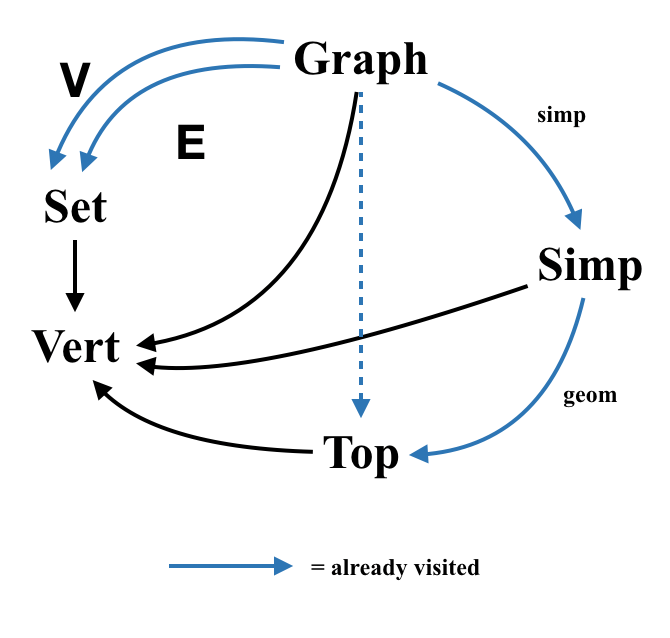
\includegraphics[width=0.5\textwidth]{Images/bigPicture.png}

\end{document}
